\section{Related Work}
\label{sec:related_work}
\par In the section \ref{sec:system_design}, it explain the prototype system of this report. The concept is to use three bundles to communicate through local communication channel or remote communication channel to build the self-adaptive system to control the house heating system. There are several similar concept consuming product on the market, they will be discussed and compared with our self-adaptive heating system in this section.

\subsection{Ninja Sphere}

\begin{figure}
	\centering    	
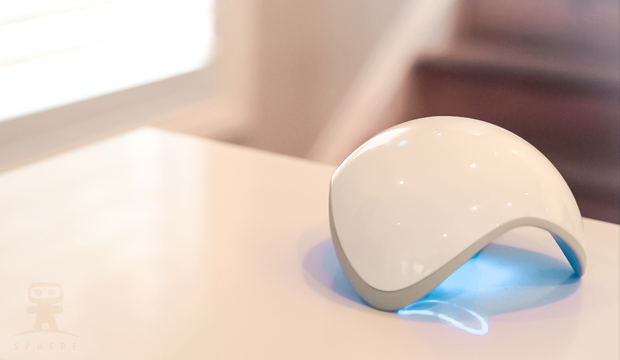
\includegraphics[width=0.90\textwidth,natwidth=610,natheight=642]{figs/ninja_sphere_gateway.png}
  	\caption{Spheramid Gateway}
  	\label{fig:ninja_sphere_gateway}
\end{figure}

\par Ninja Sphere\cite{NINJA_SPHERE} is a kickstarter\cite{kickstarter} project just currently founded on the kickstarter website. It is a next generation control of the environment with accurate in-home location data and a gesture control interface. Ninja Sphere learns about the user and user environment. It uses data from sensors and actuators to build a model that can inform user if something is out of place. It can monitor temperature,lighting,energy usage, user and even user pets' presence, and anything else user connect to their sphere. By using data from user's devices,environment and location, ninja sphere is able to advise you intelligently and give user control only when user need it. Like our prototype project, the devices connected with Ninja Sphere is 'dump' device, there are no directly communication between these 'dump' device, every device only care about their own responsible function.
The developer of the Ninja Sphere has released the supported devices for the system to connect with in Figure\ref{fig:ninja_sphere_conect_devices}.

\begin{figure}
	\centering    	
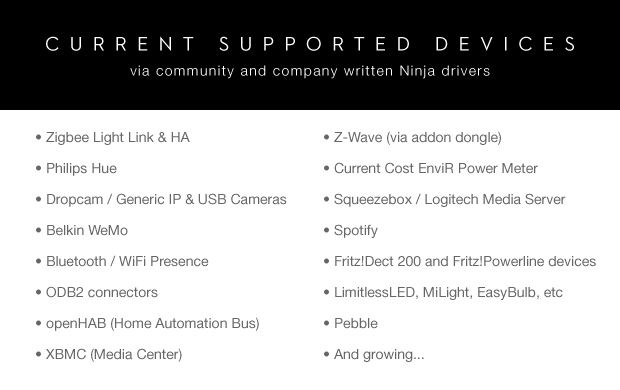
\includegraphics[width=0.90\textwidth,natwidth=610,natheight=642]{figs/ninja_sphere_conect_devices.png}
  	\caption{Ninja Sphere Current Supported Devices}
  	\label{fig:ninja_sphere_conect_devices}
\end{figure}

\par And according to Ninja Sphere system architecture in Figure \ref{fig:ninja_sphere_system}, the main control component in the system is Spheramid Gateway\ref{fig:ninja_sphere_gateway}, it is the main service component to be used for other connected devices communicate with. In our project system, it will the same as heater binding to bind one heater device and one temperature sensor as a service block in the system. Although in the prototype of this report is only based on internet communication not like the Spheramid Gateway has Wifi, Bluetooth Classic \& Low Energy, ZigBee and USB communication method, the basic concept is the same to be as a main communication bridge to cooperate with other component in the system.

\begin{figure}
	\centering    	
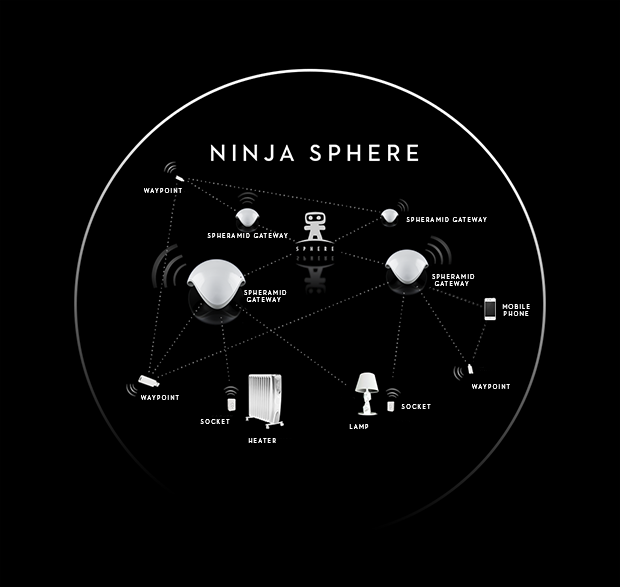
\includegraphics[width=0.90\textwidth,natwidth=610,natheight=642]{figs/ninja_sphere_system.png}
  	\caption{Ninja Sphere System Architecture}
  	\label{fig:ninja_sphere_system}
\end{figure}

\par For Ninja Sphere system, the user can user their smart phone or wearable smart device (like Google Glass or smart watch) to control and get notification from other daily using devices in the house. For example, user Adam left home and forget to turn off the heater, then the Ninja Sphere system will make the decision send the notification to Adam's smart device to ask user if they forgot to turn off the heater. Once Adam think he forgot to turn off the heater, then he can use the smart device to send turn off command to the system, after that the system will send the command to turn off the running heater in the house. And in current project of this report, the user case is almost the same except the notification and cooperate with smart device function is not implemented in current phase.
\par In the system of this report, the system has some configuration value from the user which can be changed by the user as well, then the other 'dump' component in the system will do the self-adaptive process when they reach the certain threshold value. The basic concept is the same as Ninja Sphere system.

\subsection{HyttaMi}

\par HyttaMi\cite{hyttami} service is a consuming product developed by DEFA AS\cite{defa}. Hyttami is a subscription based service including GSM subscription for product costs associated with the use of the service , and it provides the easiest and most effective way for remote control and monitoring of electricity, heating and alarm in the cabin.
\par HyttaMi gives the user a safe and secure solution with full control of heating and alarms in the house . It is very easy to control and monitor both heat , temperature and alarm via the internet , telephone and sms.
\par The main function HyttaMi has are:
\begin{itemize}
	\item Turn on or off the heat using a text message
	\item Check the status of the cabin using a text message
	\item Turn on or off the heat using the internet
	\item Check the status of the cabin using the internet
	\item Turn on or off the heat using a normal phone
\end{itemize}
\par According to the system architecture in Figure \ref{fig:hyttami_system}, the working process is also a self-adaptive and user controlling system. Although HyttaMi provides more services than heating control system, other services compare to heating control system has the same basic working logic which is also the same as the prototype system in this report.

\begin{figure}
	\centering    	
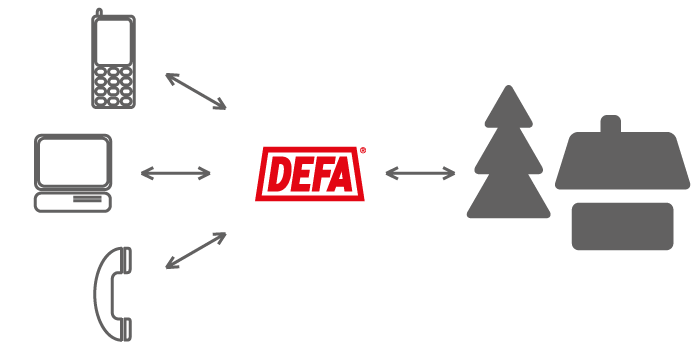
\includegraphics[width=0.90\textwidth,natwidth=610,natheight=642]{figs/hyttami_system.png}
  	\caption{HyttaMi System Architecture}
  	\label{fig:hyttami_system}
\end{figure}

\par The normal user case of HyttaMi could be like, user Eva wants to go to her cabin this weekend, but she still needs to work in the weekday, so originally there is no way for her to make the heating system working in her cabin unless she goes there. But now by using Hyttami, she can just use her phone to send some sms message to the correct number, then the system will turn on the heating system and wait her coming to enjoy the cabin weekend. This working process is also implement in the system of this report. Once user binds the heater device and temperature sensor together, it initially start the heating logic, then the temperature sensor would send current temperature value to the control component, according to certain threshold user set before, the heating would be working to reach the temperature threshold. Moreover since the heater binder, heater device and temperature sensor are not communicate directly, they all communicate with the Hydna service, then each bundle can be initiated and allocated resources in different places. So the remote control process is also possible in the current prototype system.

\subsection{Feedback from Related Work}
\par After researching about the related work in the consumer market, it is quite interesting to notice that there are quite a few product have the same working process and concept as the system of this report. And since the development of the smart devices, more and more the system provide the service which mainly communicated with smart device component in the reality.
\par Because of the time limitation of the system in this report, the potential function of this kind system which are communicated with smart devices has not been implemented yet. But the work flow to implement this important function will not be so hard in the future work of this system since currently all the communication are based on the internet and the main advantage of the smart device is to keep the user on the internet as long as possible.
\par It is really promising feature if the cooperation of smart devices are done for this project. 
